\documentclass{beamer}

\title{\Huge Matrix Project}
\subtitle{\huge EE-1390}

\author{Sunny Manne \and Aditya Singh \\MS18BTECH11015 \and CS18BTECH11048}
%\author{roll(MS18BTECH11015) \and roll(CS18BTECH11048)}


\usetheme{Singapore}

\begin{document}
\begin{frame}
  \titlepage
\end{frame}
\begin{frame}{\LARGE Geometrical Question}{question 22}
	
	{\Large If an equlateral triangle, having centroid at the origin, has a        	side along the line \textbf{x + y = 2}, then find the area of this triangle.}
	

\end{frame}

\begin{frame}{\LARGE Matrix Transformation}
	\begin{itemize}
	
	\item {A line can be written in the form $$\textbf{n}\cdot(\textbf{r} - \textbf{a}) = 0$$}
	
	\item {where \textbf{n} is normal vector, \textbf{r} is position vector of points on the line, and \textbf{a} is position vector of any known point lying on the line }
	

	\end{itemize}

\end{frame}

\begin{frame}{\LARGE Matrix Transformation}{contd...}
	\begin{itemize}
	
	\item {In our case  \textbf{n} is $(\begin{array}{cc}1 & 1
	
	\end{array})
	$ and \textbf{r} is $(\begin{array}{c}x \\ y
	
	\end{array})
	$}
	
	\item {and  $\textbf{n}\cdot \textbf{a} = 2$}
	
	\item {hence equation in terms of matrix is: $(\begin{array}{cc}1 & 1
	
	\end{array})\cdot \textbf{r} = 2
	$ }
	

	\end{itemize}

\end{frame}

\begin{frame}{\LARGE Solution in terms of Matrix}
\begin{itemize}
\item {let the centroid(origin) be G = $(\begin{array}{cc}0 & 0
	
	\end{array})$,\\ and the point of intersection of median with given base be X}
\item {To find X following system of equation needs to be solved:\\ 
$\textbf{n1}\cdot\textbf{r} = \textbf{n1}\cdot\textbf{a}$  and  \\ 
$\textbf{n2}\cdot\textbf{r} = \textbf{n2}\cdot\textbf{G}$}

\item {where \textbf{n1} = $(\begin{array}{cc}1 & 1\end{array})$, and \\
\textbf{n2} =  $(\begin{array}{cc}0 & -1 \\ 1 & 0
	
	\end{array})(\begin{array}{cc}1 & 1
	
	\end{array})^T
	$}
\end{itemize}

\end{frame}

\begin{frame}{Solution contd...}
\begin{itemize}
	\item {Therefore the sysytem of the equation can be written as: \\
	 \textbf{X} = \textbf{inv(N)}*\textbf{C} }
	\item {Here N = $(\begin{array}{cc}\textbf{n1}\\\textbf{n2} \end{array})$ or $N = (\begin{array}{cc}1 & 1 \\ 1 & -1\end{array})$
	\\ , and}
	\item {Here C = $(\begin{array}{cc}\textbf{n1} \cdot \textbf{a}\\\textbf{n2} \cdot \textbf{G} \end{array})$ or $C = (\begin{array}{cc}2\\0 \end{array})$}
	\item {solving the equations we get X =  $(\begin{array}{c}1\\1
	\end{array})$}

\end{itemize}
\end{frame}

\begin{frame}{\LARGE Graph}
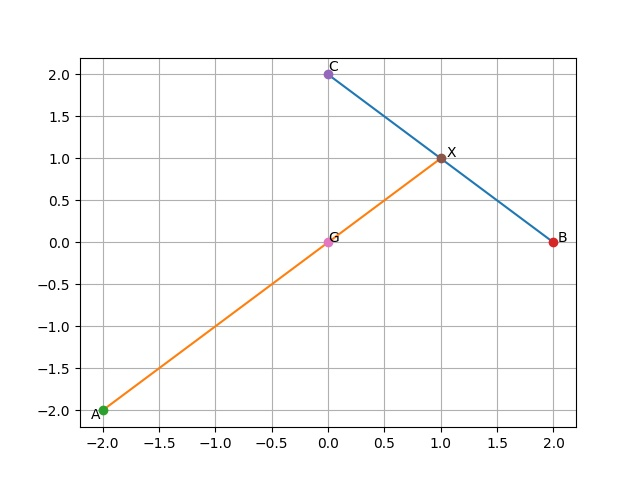
\includegraphics[scale=0.5]{figure1}
\end{frame}


\end{document}
